
\typeout{************************************************}
\typeout{Chapter 11 Back to Power Series}
\typeout{************************************************}
%
\begin{chapterptx}{Back to Power Series}{}{Back to Power Series}{}{}{x:chapter:PowerSeriesRedux}
	%
	%
	\typeout{************************************************}
	\typeout{Section 11.1 Uniform Convergence}
	\typeout{************************************************}
	%
	\begin{sectionptx}{Uniform Convergence}{}{Uniform Convergence}{}{}{x:section:PowerSeriesRedux-UnifConv}
		We have developed precise analytic definitions of the convergence of a sequence and continuity of a function and we have used these to prove the EVT and IVT for a continuous function. We will now draw our attention back to the question that originally motivated these definitions, ``Why are Taylor series well behaved, but Fourier series are not necessarily?'' More precisely, we mentioned that whenever a power series converges then whatever it converged to was continuous. Moreover, if we differentiate or integrate these series term by term then the resulting series will converge to the derivative or integral of the original series. This was not always the case for Fourier series. For example consider the function%
		\begin{align*}
			f(x) \amp = \frac{4}{\pi}\left(\sum_{k=0}^\infty\frac{(-1)^k}{2k+1}\cos\left((2k+1)\pi x\right)\right)\\
			\amp = \frac{4}{\pi}\left(\cos(\pi x)-\frac13\cos(3\pi x)+\frac15 (5\pi x)-\ldots\right)\text{.}
		\end{align*}
		%
		\par
		We have seen that the graph of \(f\) is given by%
		\begin{image}{0.075}{0.85}{0.075}%
			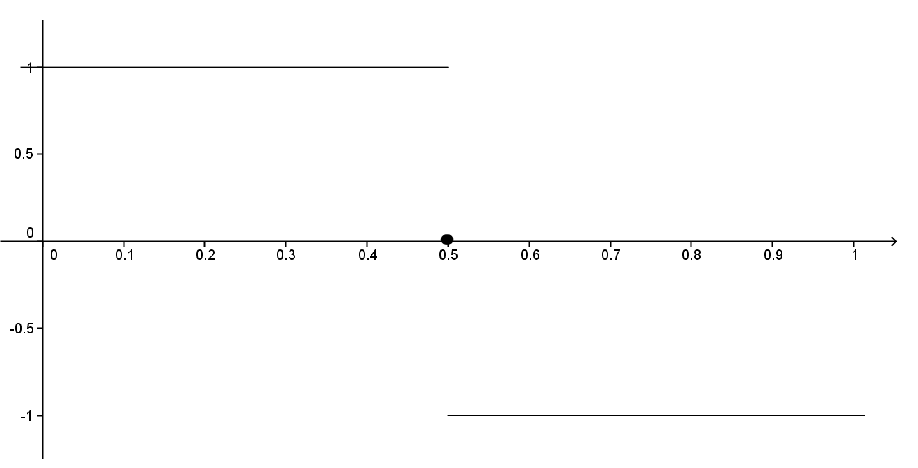
\includegraphics[width=\linewidth]{external/images/Ch7fig1.png}
		\end{image}%
		If we consider the following sequence of functions%
		\begin{align*}
			f_1(x)=\amp \frac{4}{\pi}\cos\left(\pi x\right)\\
			f_2(x)=\amp \frac{4}{\pi}\left(\cos \left(\pi x\right)-\frac{1}{3}\cos\left( 3\pi x\right)\right)\\
			f_3(x)=\amp \frac{4}{\pi}\left(\cos\left(\pi x\right)-\frac{1}{3}\cos\left(3\pi x\right)+\frac{1}{5}\cos\left(5\pi x\right)\right)\\
			\amp \vdots
		\end{align*}
		we see the sequence of continuous functions \(\left(f_n\right)\) converges to the non-continuous function \(f\) for each real number \(x\). This didn't happen with Taylor series. The partial sums for a Taylor series were polynomials and hence continuous but what they converged to was continuous as well.%
		\par
		The difficulty is quite delicate and it took mathematicians a while to determine the problem. There are two very subtly different ways that a sequence of functions can converge: pointwise or uniformly. This \index{Abel, Niels Henrik} distinction was touched upon by Niels Henrik Abel (1802-1829) in 1826 while studying the domain of convergence of a power series. However, the necessary formal definitions were not made explicit until Weierstrass \index{Weierstrass, Karl} did it in his 1841 paper \textit{Zur Theorie der Potenzreihen} \emph{(On the Theory of Power Series)}. This was published in his collected works in 1894.%
		\par
		It will be instructive to take a look at an argument that doesn't quite work before looking at the formal definitions we will need. In 1821 Augustin Cauchy \index{Cauchy, Augustin} ``proved'' that the infinite sum of continuous functions is continuous. Of course, it is obvious (to us) that this is not true because we've seen several counterexamples. But Cauchy, who was a first rate mathematician was so sure of the correctness of his argument that he included it in his textbook on analysis, \textit{Cours d'analyse} (1821).%
		\begin{problem}{}{x:problem:prob_Cauchy_s_incorrect_proof}%
			\index{Cauchy, Augustin!Cauchy's flawed proof that the limit of continuous functions is continuous}\index{continuity!Cauchy's flawed proof that the limit of continuous functions is continuous} Find the flaw in the following ``proof'' that \(f\) is also continuous at \(a\).%
			\par
			Suppose \(f_1, f_2, f_3, f_4 \ldots\) are all continuous at \(a\) and that \(\sum_{n=1}^\infty f_n=f\). Let \(\eps>0\). Since \(f_n\) is continuous at \(a\), we can choose \(\delta_n>0\) such that if \(\abs{x-a}\lt \delta_n\), then \(\abs{f_n(x)-f_n(a)}\lt \frac{\eps}{2^n}\). Let \(\delta=\inf(\delta_1,\delta_2,\delta_3,\ldots)\). If \(\abs{x-a}\lt \delta\) then%
			\begin{align*}
				\abs{f(x)-f(a)} \amp =  \abs{\sum_{n=1}^\infty f_n(x)  -  \sum_{n=1}^\infty f_n(a) }\\
				\amp = \abs{\sum_{n=1}^\infty \left(f_n(x)-f_n(a)\right) }\\
				\amp \le \sum_{n=1}^\infty \abs{f_n(x)-f_n(a) }\\
				\amp \le \sum_{n=1}^\infty \frac{\eps}{2^n}\\
				\amp \le \eps\sum_{n=1}^\infty \frac{1}{2^n}\\
				\amp =   \eps\text{.}
			\end{align*}
			%
			\par
			Thus \(f\) is continuous at \(a\).%
		\end{problem}
		\begin{definition}{}{x:definition:def_PointwiseConvergence}%
			\index{convergence!of a series!pointwise} Let \(S\) be a subset of the real number system and let \(\left(f_n\right)=\left(f_1,f_2,f_3,\,\ldots\right)\) be a sequence of functions defined on \(S\). Let \(f\) be a function defined on \(S\) as well. We say that  \(\left(f_n\right)\) \alert{converges to \(f\) pointwise on \(S\)} provided that for all \(x\in S\), the sequence of real numbers \(\left(f_n(x)\right)\) converges to the number \(f(x)\). In this case we write\(\,f_n\ptwise f\) on \(S\).%
		\end{definition}
		Symbolically, we have \(f_n\ptwise f\text{ on } S\Leftrightarrow \forall\,x\in S,\forall\ \eps>0,\,\exists\ N\) such that \(\left(n>N \Rightarrow|f_n(x)-f(x)|\lt \eps\right)\).%
		\par
		This is the type of convergence we have been observing to this point. By contrast we have the following new definition.%
		\begin{definition}{}{x:definition:def_UniformConvergence}%
			\index{uniform convergence} Let \(S\) be a subset of the real number system and let \(\left(f_n\right)=\left(f_1,f_2,f_3,\,\ldots\right)\) be a sequence of functions defined on \(S\). Let \(f\) be a function defined on \(S\) as well. We say that \(\left(f_n\right)\) \alert{converges to \(f\) uniformly on \(S\)} provided \(\forall\ \eps>0,\,\exists\ N\) such that \(n>N\Rightarrow|f_n(x)-f(x)|\lt \eps\text{ , } \forall\
			x\in S\).%
			\par
			In this case we write \(f_n\unif f\) on \(S\).%
		\end{definition}
		The difference between these two definitions is subtle. In pointwise convergence, we are given a fixed \(x\in S\) and an \(\eps>0\). Then the task is to find an \(N\) that works for that particular \(x\) and \(\eps\). In uniform convergence, one is given \(\eps>0\) and must find a single \(N\) that works for that particular \(\eps\) but also simultaneously (uniformly) for all \(x\in S\). Clearly uniform convergence implies pointwise convergence as an \(N\) which works uniformly for all \(x\), works for each individual \(x\) also. However the reverse is not true. This will become evident, but first consider the following example.%
		\begin{problem}{}{x:problem:prob_uniform_convergence}%
			Let \(0\lt b\lt 1\) and consider the sequence of functions \(\left(f_n\right)\) defined on \([0,b]\) by \(f_n(x)=x^n\). Use the definition to show that \(f_n\unif 0\) on \([0,b]\).%
			\par\smallskip%
			\noindent\textbf{\blocktitlefont Hint}.\hypertarget{g:hint:idp277}{}\quad{}\(|x^n-0|=x^n\leq b^n\).%
		\end{problem}
		Uniform convergence is not only dependent on the sequence of functions but also on the set \(S\). For example, the sequence \(\left(f_n(x)\right)=\left(x^n\right)_{n=0}^\infty\) of \hyperref[x:problem:prob_uniform_convergence]{Problem~{\xreffont\ref{x:problem:prob_uniform_convergence}}} does not converge uniformly on \([0,1]\). We could use the negation of the definition to prove this, but instead, it will be a consequence of the following theorem.%
		\begin{theorem}{}{}{x:theorem:thm_UnifConv-_Continuity}%
			\index{uniform convergence!continuous functions and}\index{continuous functions!uniform convergence and}\index{continuous functions!uniform limit of continuous functions is continuous} Consider a sequence of functions \(\left(f_n\right)\) which are all continuous on an interval \(I\). Suppose \(f_n\unif f\) on \(I\). Then \(f\) must be continuous on \(I\).%
		\end{theorem}
		\begin{proof}{Sketch of Proof.}{g:proof:idp278}
			Let \(a\in I\) and let \(\eps>0\). The idea is to use uniform convergence to replace \(f\) with one of the known continuous functions \(f_n\). Specifically, by uncancelling, we can write%
			\begin{align*}
				\left|f(x)-f(a)\right|\amp =\left|f(x)-f_n(x)+f_n(x)-f_n(a)+f_n(a)-f(a)\right|\\
				\amp \leq \left|f(x)-f_n(x)\right|+\left|f_n(x)-f_n(a)\right|+\left|f_n(a)-f(a)\right|
			\end{align*}
			%
			\par
			If we choose \(n\) large enough, then we can make the first and last terms as small as we wish, noting that the uniform convergence makes the first term uniformly small for all \(x\). Once we have a specific \(n\), then we can use the continuity of \(f_n\) to find a \(\delta>0\) such that the middle term is small whenever \(x\) is within \(\delta\) of \(a\).%
		\end{proof}
		\begin{problem}{}{g:problem:idp279}%
			\index{uniform convergence!continuous functions and} Provide a formal proof of \hyperref[x:theorem:thm_UnifConv-_Continuity]{Theorem~{\xreffont\ref{x:theorem:thm_UnifConv-_Continuity}}} based on the above ideas.%
		\end{problem}
		\begin{problem}{}{g:problem:idp280}%
			\index{\(x^n\)!converges pointwise on \([0,1]\)}\index{pointwise convergence}\index{\(x^n\) converges pointwise on \([0,1]\)} Consider the sequence of functions \(\left(f_n\right)\) defined on \([0,1]\) by \(f_n(x)=x^n\). Show that the sequence converges to the function%
			\begin{equation*}
				f(x)= \begin{cases}0\amp \text{ if  } x\in[0,1)\\ 1\amp \text{ if } x=1 \end{cases}
			\end{equation*}
			pointwise on \(\,[0,1]\), but not uniformly on \([0,1]\).%
		\end{problem}
		Notice that for the Fourier series at the beginning of this chapter,%
		\begin{equation*}
			f(x)=\frac{4}{\pi}\left(\cos\left(\frac{\pi}{2}x\right)-\frac{1}{3}\cos\left( 3\pi x\right)+\frac{1}{5}\cos\left(5\pi x\right)-\frac{1}{7}\cos\left(7\pi x\right)+\cdots\right)
		\end{equation*}
		the convergence cannot be uniform on \((-\infty,\infty)\), as the function \(f\) is not continuous. This never happens with a power series, since they converge to continuous functions whenever they converge. We will also see that uniform convergence is what allows us to integrate and differentiate a power series term by term.%
	\end{sectionptx}
	%
	%
	\typeout{************************************************}
	\typeout{Section 11.2 Uniform Convergence: Integrals and Derivatives}
	\typeout{************************************************}
	%
	\begin{sectionptx}{Uniform Convergence: Integrals and Derivatives}{}{Uniform Convergence: Integrals and Derivatives}{}{}{x:section:PowerSeriesRedux-UnifConv-IntsAndDerivs}
		\begin{introduction}{}%
			We saw in the previous section that if \(\left(f_n\right)\) is a sequence of continuous functions which converges uniformly to \(f\) on an interval, then \(f\) must be continuous on the interval as well. This was not necessarily true if the convergence was only pointwise, as we saw a sequence of continuous functions defined on \((-\infty,\infty)\) converging pointwise to a Fourier series that was not continuous on the real line. Uniform convergence guarantees some other nice properties as well.%
			\begin{theorem}{}{}{x:theorem:th_UniformIntegralConvergence}%
				\index{uniform convergence!integration and} Suppose \(f_n\) and \(f\) are integrable and \(f_n\unif f\) on \([a,b]\). Then%
				\begin{equation*}
					\lim_{n\rightarrow\infty}\int_{x=a}^b f_n(x)\dx{ x}=\int_{x=a}^bf(x)\dx{ x}. {}
				\end{equation*}
				%
			\end{theorem}
			\begin{problem}{}{g:problem:idp281}%
				\index{uniform convergence!integration and} Prove \hyperref[x:theorem:th_UniformIntegralConvergence]{Theorem~{\xreffont\ref{x:theorem:th_UniformIntegralConvergence}}}.%
				\par\smallskip%
				\noindent\textbf{\blocktitlefont Hint}.\hypertarget{g:hint:idp282}{}\quad{}For \(\eps>0\), we need to make \(|f_n(x)-f(x)|\lt \frac{\eps}{b-a}\), for all \(x\in[a,b]\).%
			\end{problem}
			Notice that this theorem is not true if the convergence is only pointwise, as illustrated by the following.%
			\begin{problem}{}{g:problem:idp283}%
				\index{convergence!pointwise convergence}\index{convergence!uniform convergence}\index{convergence!pointwise vs. uniform convergence} Consider the sequence of functions \(\left(f_n\right)\) given by%
				\begin{equation*}
					f_n(x)= \begin{cases}n\amp \text{ if } x\in\left(0,\frac{1}{n}\right)\\ 0\amp \text{ otherwise } \end{cases} \text{.}
				\end{equation*}
				%
				\begin{enumerate}[label=(\alph*)]
					\item{}Show that \(f_n\ptwise 0\) on \([0,1]\), but \(\limit{n}{\infty}{\int_{x=0}^1f_n(x)\dx{ x}\neq\int_{x=0}^10\dx{ x}.}\)%
					\item{}Can the convergence be uniform? Explain.%
				\end{enumerate}
				%
			\end{problem}
			Applying this result to power series we have the following.%
			\begin{aside}{}{g:aside:idp284}%
				Notice that we must explicitly assume uniform convergence. This is because we have not \emph{yet} proved that power series actually do converge uniformly.%
			\end{aside}
			\begin{corollary}{}{}{x:corollary:cor_IntConvUni}%
				If \(\sum_{n=0}^\infty a_nx^n\) converges uniformly to \(f\) on an interval containing \(0\) and \(x\) then \(\int_{t=0}^xf(t)\dx{ t}=\sum_{n=0}^\infty\left(\frac{a_n}{n+1}x^{n+1}\right)\).%
			\end{corollary}
			\begin{problem}{}{g:problem:idp285}%
				\index{power series!term by term integral of} Prove \hyperref[x:corollary:cor_IntConvUni]{Corollary~{\xreffont\ref{x:corollary:cor_IntConvUni}}}.%
				\par\smallskip%
				\noindent\textbf{\blocktitlefont Hint}.\hypertarget{g:hint:idp286}{}\quad{}Remember that%
				\begin{equation*}
					\displaystyle \sum_{n=0}^\infty f_n(x) = \lim_{N\rightarrow\infty}\sum_{n=0}^N f_n(x). 
				\end{equation*}
				%
			\end{problem}
			Surprisingly, the issue of term-by-term differentiation depends not on the uniform convergence of \(\left(f_n\right)\), but on the uniform convergence of \(\left(f^\prime_n\right)\). More precisely, we have the following result.%
			\begin{theorem}{}{}{x:theorem:thm_UniformDerivativeConvergence}%
				\index{pointwise convergence!derivative and}%
				\index{differentiation!of the pointwise limit of functions}%
				Suppose for every \(n\in\NN\) \(f_n\) is differentiable, \(f_n^\prime\) is continuous, \(f_n\ptwise f\), and \(f_n^\prime\unif g\) on an interval, \(I\).  Then \(f\) is differentiable and \(f^\prime = g\) on \(I\).%
			\end{theorem}
			\begin{problem}{}{g:problem:idp287}%
				Prove \hyperref[x:theorem:thm_UniformDerivativeConvergence]{Theorem~{\xreffont\ref{x:theorem:thm_UniformDerivativeConvergence}}}.%
				\par\smallskip%
				\noindent\textbf{\blocktitlefont Hint}.\hypertarget{g:hint:idp288}{}\quad{}Let \(a\) be an arbitrary fixed point in \(I\) and let \(x\in
				I\).  By the Fundamental Theorem of Calculus, we have%
				\begin{equation*}
					\int_{t=a}^x f^\prime_n(t)\dx{ t}=f_n(x)-f_n(a)\text{.}
				\end{equation*}
				Take the limit of both sides and differentiate with respect to \(x\).%
			\end{problem}
			As before, applying this to power series gives the following result.%
			\begin{corollary}{}{}{x:corollary:cor_UniformConvergenceDerivative}%
				If \(\sum_{n=0}^\infty a_nx^n\) converges pointwise to \(f\) on an interval containing \(0\) and \(x\) and \(\sum_{n=1}^\infty a_nnx^{n-1}\) converges uniformly on an interval containing \(0\) and \(x\), then \(f^\prime(x)=\sum_{n=1}^\infty a_nnx^{n-1}\).%
			\end{corollary}
			\begin{problem}{}{g:problem:idp289}%
				\index{power series!term by term derivative of}\index{differentiation!term by term differentiation of power series} Prove \hyperref[x:corollary:cor_UniformConvergenceDerivative]{Corollary~{\xreffont\ref{x:corollary:cor_UniformConvergenceDerivative}}}.%
			\end{problem}
			The above results say that a power series can be differentiated and integrated term-by-term as long as the convergence is uniform. Fortunately it is, in general, true that when a power series converges the convergence of it and its integrated and differentiated series is also uniform (almost).%
			\par
			However we do not yet have all of the tools necessary to see this. To build these tools requires that we return briefly to our study, begun in \hyperref[x:chapter:Convergence]{Chapter~{\xreffont\ref{x:chapter:Convergence}}}, of the convergence of sequences.%
		\end{introduction}%
		%
		%
		\typeout{************************************************}
		\typeout{Subsection 11.2.1 Cauchy Sequences}
		\typeout{************************************************}
		%
		\begin{subsectionptx}{Cauchy Sequences}{}{Cauchy Sequences}{}{}{g:subsection:idp290}
			Knowing that a sequence or a series converges and knowing what it converges to are typically two different matters. For example, we know that \(\sum_{n=0}^\infty\frac{1}{n!}\)and \(\sum_{n=0}^\infty\frac{1}{n!\,n!}\) both converge. The first converges to \(e\), which has meaning in other contexts. We don't know what the second one converges to, other than to say it converges to \(\sum_{n=0}^\infty\frac{1}{n!\,n!}\). In fact, that question might not have much meaning without some other context in which \(\sum_{n=0}^\infty\frac{1}{n!\,n!}\) arises naturally. Be that as it may, we need to look at the convergence of a series (or a sequence for that matter) without necessarily knowing what it might converge to. We make the following definition.%
			\begin{definition}{}{x:definition:def_CauchySequence}%
				\index{sequences!Cauchy sequences} Let \(\left(s_n\right)\) be a sequence of real numbers. We say that \(\left(s_n\right)\)is a \terminology{Cauchy sequence} if for any \(\eps>0\), there exists a real number \(N\) such that if \(m,n>N\), then \(|s_m-s_n|\lt \eps\).%
			\end{definition}
			Notice that this definition says that the terms in a Cauchy sequence get arbitrarily close to each other and that there is no reference to getting close to any particular fixed real number. Furthermore, you have already seen lots of examples of Cauchy sequences as illustrated by the following result.%
			\begin{theorem}{}{}{x:theorem:thm_Converge-_Cauchy}%
				\index{sequences!convergence}\index{convergence!of a sequence!implies Cauchy sequence} Suppose \(\left(s_n\right)\) is a sequence of real numbers which converges to \(s\). Then \(\left(s_n\right)\) is a Cauchy sequence.%
			\end{theorem}
			Intuitively, this result makes sense. If the terms in a sequence are getting arbitrarily close to \(s\), then they should be getting arbitrarily close to each other. This is the basis of the proof.%
			\begin{aside}{}{g:aside:idp291}%
				But the converse isn't nearly as clear. In fact, it isn't true in the rational numbers.%
			\end{aside}
			\begin{problem}{}{g:problem:idp292}%
				Prove \hyperref[x:theorem:thm_Converge-_Cauchy]{Theorem~{\xreffont\ref{x:theorem:thm_Converge-_Cauchy}}}.%
				\par\smallskip%
				\noindent\textbf{\blocktitlefont Hint}.\hypertarget{g:hint:idp293}{}\quad{}\(|s_m-s_n|=|s_m-s+s-s_n|\leq|s_m-s\mathopen|+|s-s_n|\).%
			\end{problem}
			So any convergent sequence is automatically Cauchy. For the real number system, the converse is also true and, in fact, is equivalent to any of our completeness axioms: the NIP, the Bolzano-Weierstrass Theorem, or the LUB Property. Thus, this could have been taken as our completeness axiom and we could have used it to prove the others. One of the most convenient ways to prove this converse is to use the Bolzano-Weierstrass Theorem. To do that, we must first show that a Cauchy sequence must be bounded. This result is reminiscent of the fact that a convergent sequence is bounded (\hyperref[x:lemma:lemma_BoundedConvergent]{Lemma~{\xreffont\ref{x:lemma:lemma_BoundedConvergent}}} of \hyperref[x:chapter:Convergence]{Chapter~{\xreffont\ref{x:chapter:Convergence}}}) and the proof is very similar.%
			\begin{lemma}{}{}{x:lemma:lemma_Cauchy-_Bounded}%
				Suppose \(\left(s_n\right)\) \(\)is a Cauchy sequence. Then there exists \(B>0\) such that \(|s_n|\leq B\) for all \(n\).%
			\end{lemma}
			\begin{problem}{}{g:problem:idp294}%
				Prove \hyperref[x:lemma:lemma_Cauchy-_Bounded]{Lemma~{\xreffont\ref{x:lemma:lemma_Cauchy-_Bounded}}}.%
				\par\smallskip%
				\noindent\textbf{\blocktitlefont Hint}.\hypertarget{g:hint:idp295}{}\quad{}This is similar to \hyperref[x:problem:prob_BoundedConvergent]{problem~{\xreffont\ref{x:problem:prob_BoundedConvergent}}} of \hyperref[x:chapter:Convergence]{Chapter~{\xreffont\ref{x:chapter:Convergence}}}. There exists \(N\) such that if \(m,n>N\)then \(|s_n-s_m|\lt 1.\), Choose a fixed \(m>N\) and let \(B=\max\left(\abs{s_1}, \abs{s_2}, \ldots, \abs{s_{\lceil N\rceil}}, \abs{s_m}+1\right)\).%
			\end{problem}
			\begin{theorem}{}{}{x:theorem:thm_Cauchy-_Converge}%
				\alert{Cauchy sequences converge}%
				\par
				\index{sequences!Cauchy sequences!convergence of} Suppose \(\left(s_n\right)\) is a Cauchy sequence of real numbers. There exists a real number \(s\) such that \(\lim_{n\rightarrow\infty}s_n=s\).%
			\end{theorem}
			\begin{proof}{Sketch of Proof.}{g:proof:idp296}
				We know that \(\left(s_n\right)\) \(\)is bounded, so by the Bolzano-Weierstrass Theorem, it has a convergent subsequence \(\left(s_{n_k}\right)\) converging to some real number \(s\). We have \(|s_n-s|=|s_n-s_{n_k}+s_{n_k}-s|\leq|s_n-s_{n_k}\mathopen|+|s_{n_k}-s|\). If we choose \(n\) and \(n_k\) large enough, we should be able to make each term arbitrarily small.%
			\end{proof}
			\begin{problem}{}{x:problem:prob_Cauchy_sequences_Cauchy_implies_convergence}%
				\index{sequences!Cauchy sequences!convergence of} Provide a formal proof of \hyperref[x:theorem:thm_Cauchy-_Converge]{Theorem~{\xreffont\ref{x:theorem:thm_Cauchy-_Converge}}}.%
			\end{problem}
			From \hyperref[x:theorem:thm_Converge-_Cauchy]{Theorem~{\xreffont\ref{x:theorem:thm_Converge-_Cauchy}}} we see that every Cauchy sequence converges in \(\RR\). Moreover the proof of this fact depends on the Bolzano-Weierstrass Theorem which, as we have seen, is equivalent to our completeness axiom, the Nested Interval Property. What this means is that if there is a Cauchy sequence which does not converge then the NIP is not true. A natural question to ask is if every Cauchy sequence converges does the NIP follow? That is, is the convergence of Cauchy sequences also equivalent to our completeness axiom? The following theorem shows that the answer is yes.%
			\begin{theorem}{}{}{x:theorem:thm_ConvCauchyEquivNIP}%
				\index{sequences!Cauchy sequences!convergence of is equivalent to the NIP} Suppose every Cauchy sequence converges. Then the Nested Interval Property is true.%
			\end{theorem}
			\begin{problem}{}{x:problem:prob_Cauchy_sequences_Cauchy_implies_NIP}%
				Prove \hyperref[x:theorem:thm_ConvCauchyEquivNIP]{Theorem~{\xreffont\ref{x:theorem:thm_ConvCauchyEquivNIP}}}.%
				\par\smallskip%
				\noindent\textbf{\blocktitlefont Hint}.\hypertarget{g:hint:idp297}{}\quad{}If we start with two sequences \(\left(x_n\right)\) and \(\left(y_n\right)\), satisfying all of the conditions of the NIP, you should be able to show that these are both Cauchy sequences.%
			\end{problem}
			\hyperref[x:problem:prob_Cauchy_sequences_Cauchy_implies_convergence]{Problems~{\xreffont\ref{x:problem:prob_Cauchy_sequences_Cauchy_implies_convergence}}} and \hyperref[x:problem:prob_Cauchy_sequences_Cauchy_implies_NIP]{Problem~{\xreffont\ref{x:problem:prob_Cauchy_sequences_Cauchy_implies_NIP}}} tell us that the following are equivalent: the Nested Interval Property, the Bolzano-Weierstrass Theorem, the Least Upper Bound Property, and the convergence of Cauchy sequences. Thus any one of these could have been taken as the completeness axiom of the real number system and then used to prove the each of the others as a theorem according to the following dependency graph:%
			\begin{image}{0}{1}{0}%
				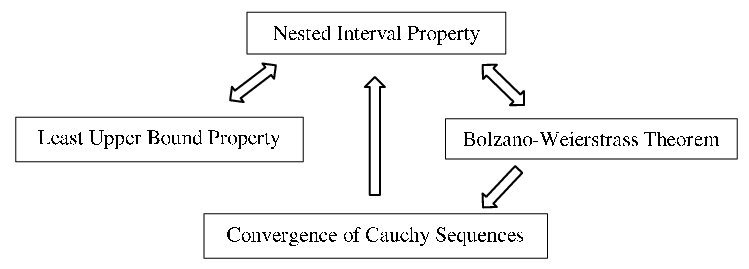
\includegraphics[width=\linewidth]{external/images/CompletenessAxioms.png}
			\end{image}%
			Since we can get from any node on the graph to any other, simply by following the implications (indicated with arrows), any one of these statements is logically equivalent to each of the others.%
			\begin{problem}{}{g:problem:idp298}%
				\index{sequences!Cauchy sequences!don't always converge in \(\QQ\)} Since the convergence of Cauchy sequences can be taken as the completeness axiom for the real number system, it does not hold for the rational number system. Give an example of a Cauchy sequence of rational numbers which does not converge to a rational number.%
			\end{problem}
			If we apply the above ideas to series we obtain the following important result, which will provide the basis for our investigation of power series.%
			\begin{theorem}{Cauchy Criterion.}{}{x:theorem:thm_CauchyCriterion}%
				\index{series!Cauchy sequences!Cauchy Criterion}%
				The series \(\sum_{k=0}^\infty a_k\) converges if and only if \(\forall \eps>0\), \(\exists N\) such that if \(m>n>N\) then \(|\sum_{k=n+1}^ma_k|\lt \eps\).%
			\end{theorem}
			\begin{problem}{}{g:problem:idp299}%
				\index{series!Cauchy Criterion} Prove the Cauchy criterion.%
			\end{problem}
			At this point several of the tests for convergence that you probably learned in calculus are easily proved.  For example:%
			\begin{problem}{}{x:problem:prob_NthTermTest}%
				\alert{The \(n\)th Term Test}%
				\par
				\index{series!\(n\)th term test}\index{divergence!of a series!\(n\)th term test} Show that if \(\sum_{n=1}^\infty a_n\) converges then \(\limit{n}{\infty}{a_n}=0\).%
			\end{problem}
			\begin{problem}{The Strong Cauchy Criterion.}{g:problem:idp300}%
				\index{series!Cauchy Criterion!Strong Cauchy criterion} Show that \(\displaystyle\sum_{k=1}^\infty a_k\) converges if and only if \(\limit{n}{\infty}{\sum_{k=n+1}^\infty a_k}=0\).%
				\par\smallskip%
				\noindent\textbf{\blocktitlefont Hint}.\hypertarget{g:hint:idp301}{}\quad{}The hardest part of this problem is recognizing that it is really about the limit of a sequence as in \hyperref[x:chapter:Convergence]{Chapter~{\xreffont\ref{x:chapter:Convergence}}}.%
			\end{problem}
			You may also recall the Comparison Test from studying series in calculus: suppose \(0\leq a_n\leq b_n\), if \(\sum b_n\) converges then \(\sum a_n\) converges. This result follows from the fact that the partial sums of \(\sum a_n\) form an increasing sequence which is bounded above by \(\sum b_n\). (See \hyperref[x:corollary:cor_IncBoundedConverge]{Corollary~{\xreffont\ref{x:corollary:cor_IncBoundedConverge}}} of \hyperref[x:chapter:IVTandEVT]{Chapter~{\xreffont\ref{x:chapter:IVTandEVT}}}.) The Cauchy Criterion allows us to extend this to the case where the terms \(a_n\) could be negative as well. This can be seen in the following theorem.%
			\begin{theorem}{}{}{x:theorem:thm_ComparisonTest}%
				\alert{Comparison Test}%
				\par
				\index{series!Comparison Test} Suppose \(|a_n|\leq b_n\) for all \(n\). If \(\sum b_n\) converges then \(\sum a_n\) also converges.%
			\end{theorem}
			\begin{problem}{}{g:problem:idp302}%
				Prove \hyperref[x:theorem:thm_ComparisonTest]{Theorem~{\xreffont\ref{x:theorem:thm_ComparisonTest}}}.%
				\par\smallskip%
				\noindent\textbf{\blocktitlefont Hint}.\hypertarget{g:hint:idp303}{}\quad{}Use the Cauchy criterion with the fact that \(\abs{\sum_{k=n+1}^ma_k}\leq\sum_{k=n+1}^m\abs{a_k}\).%
			\end{problem}
			The following definition is of marked importance in the study of series.%
			\begin{definition}{}{x:definition:AbsoluteConvergence}%
				\alert{Absolute Convergence}%
				\par
				\index{convergence!of a series!absolute} Given a series \(\sum a_n\), the series \(\sum|a_n|\) is called the \textbraceleft{}absolute series\textbraceright{} of \(\sum\boldsymbol{a}_{\boldsymbol{n}}\) and if \(\sum|a_n|\)converges then we say that \(\sum\boldsymbol{a}_{\boldsymbol{n}}\) converges absolutely.%
			\end{definition}
			The significance of this definition comes from the following result.%
			\begin{corollary}{}{}{x:corollary:cor_AbsConv-_Conv}%
				If \(\sum a_n\) converges absolutely, then \(\sum a_n\) converges.%
			\end{corollary}
			\begin{problem}{}{g:problem:idp304}%
				\index{convergence!of a series!absolute convergence implies convergence} Show that \hyperref[x:corollary:cor_AbsConv-_Conv]{Corollary~{\xreffont\ref{x:corollary:cor_AbsConv-_Conv}}} is a direct consequence of \hyperref[x:theorem:thm_ComparisonTest]{Theorem~{\xreffont\ref{x:theorem:thm_ComparisonTest}}}.%
			\end{problem}
			\begin{problem}{}{g:problem:idp305}%
				\index{series!absolute convergence of!vs. the absolute value of a series} If \(\sum_{n=0}^\infty|a_n|=s\), then does it follow that \(s=|\sum_{n=0}^\infty a_n|\)? Justify your answer. What can be said?%
			\end{problem}
			The converse of \hyperref[x:corollary:cor_AbsConv-_Conv]{Corollary~{\xreffont\ref{x:corollary:cor_AbsConv-_Conv}}} is not true as evidenced by the series \(\sum_{n=0}^\infty\frac{(-1)^n}{n+1}\). As we noted in \hyperref[x:chapter:PowerSeriesQuestions]{Chapter~{\xreffont\ref{x:chapter:PowerSeriesQuestions}}}, this series converges to ln \(2\). However, its absolute series is the Harmonic \index{series!Harmonic Series} Series which diverges. Any such series which converges, but not absolutely, is said to \alert{converge conditionally}. Recall also that in \hyperref[x:chapter:PowerSeriesQuestions]{Chapter~{\xreffont\ref{x:chapter:PowerSeriesQuestions}}}, we showed that we could rearrange the terms of the series \(\sum_{n=0}^\infty\frac{(-1)^n}{n+1}\) to make it converge to any number we wished. We noted further that all rearrangements of the series \(\sum_{n=0}^\infty\frac{(-1)^n}{\left(n+1\right)^2}\) converged to the same value. The difference between the two series is that the latter converges absolutely whereas the former does not. Specifically, we have the following result.%
			\begin{theorem}{}{}{x:theorem:thm_RearrageAbsConv}%
				\index{series!rearrangements}\index{series!absolute convergence of!rearrangements} Suppose \(\sum a_n\) converges absolutely and let \(s=\sum_{n=0}^\infty a_n\). Then any rearrangement of \(\sum a_n\) must converge to \(s\).%
			\end{theorem}
			\begin{proof}{Sketch of Proof.}{g:proof:idp306}
				We will first show that this result is true in the case where \(a_n\geq 0\). If \(\sum b_n\) represents a rearrangement of \(\sum a_n\), then notice that the sequence of partial sums \(\left(\sum_{k=0}^nb_k\right)_{n=0}^\infty\)is an increasing sequence which is bounded by \(s\). By \hyperref[x:corollary:cor_IncBoundedConverge]{Corollary~{\xreffont\ref{x:corollary:cor_IncBoundedConverge}}} of \hyperref[x:chapter:IVTandEVT]{Chapter~{\xreffont\ref{x:chapter:IVTandEVT}}}, this sequence must converge to some number \(t\) and \(t\leq s\). Furthermore \(\sum a_n\) is also a rearrangement of \(\sum b_n\). Thus the result holds for this special case. (Why?) For the general case, notice that \(a_n=\frac{|a_n\mathopen|+a_n}{2}-\frac{|a_n\mathopen|-a_n}{2}\) and that \(\sum\frac{|a_n\mathopen|+a_n}{2}\) and \(\sum\frac{|a_n\mathopen|-a_n}{2}\) are both convergent series with nonnegative terms. By the special case \(\sum\frac{|b_n\mathopen|+b_n}{2}=\) \(\sum\frac{|a_n\mathopen|+a_n}{2}\) and \(\sum\frac{|b_n\mathopen|-b_n}{2}=\) \(\sum\frac{|a_n\mathopen|-a_n}{2}\).%
			\end{proof}
			\begin{problem}{}{g:problem:idp307}%
				\index{series!absolute convergence of!rearrangements} Fill in the details and provide a formal proof of \hyperref[x:theorem:thm_RearrageAbsConv]{Theorem~{\xreffont\ref{x:theorem:thm_RearrageAbsConv}}}.%
			\end{problem}
		\end{subsectionptx}
	\end{sectionptx}
	%
	%
	\typeout{************************************************}
	\typeout{Section 11.3 Radius of Convergence of a Power Series}
	\typeout{************************************************}
	%
	\begin{sectionptx}{Radius of Convergence of a Power Series}{}{Radius of Convergence of a Power Series}{}{}{x:section:PowerSeriesRedux-RadiusOfConv}
		We've developed enough machinery to look at the convergence of power series. The fundamental result is the following theorem due to Abel.%
		\begin{theorem}{}{}{x:theorem:thm_RadiusOfConvergence}%
			\index{power series!converge inside radius of convergence} Suppose \(\sum_{n=0}^\infty a_nc^n\) converges for some nonzero real number \(c\). Then \(\sum_{n=0}^\infty a_nx^n\) converges absolutely for all \(x\) such that \(|x|\lt |c|\).%
		\end{theorem}
		To prove \hyperref[x:theorem:thm_RadiusOfConvergence]{Theorem~{\xreffont\ref{x:theorem:thm_RadiusOfConvergence}}} first note that by \hyperref[x:problem:prob_NthTermTest]{Problem~{\xreffont\ref{x:problem:prob_NthTermTest}}}, \(\limit{n}{\infty}{a_nc^n}=0\). Thus \(\left(a_nc^n\right)\) is a bounded sequence. Let \(B\) be a bound: \(\abs{a_nc^n}\le B\). Then%
		\begin{equation*}
			\abs{a_nx^n}=\abs{a_nc^n\cdot\left(\frac{x}{c}\right)^n}\leq B\abs{\frac{x}{c}}^n\text{.}
		\end{equation*}
		%
		\par
		We can now use the comparison test.%
		\begin{problem}{}{g:problem:idp308}%
			\index{power series!the radius of convergence}\index{convergence!the radius of convergence of a power series} Prove \hyperref[x:theorem:thm_RadiusOfConvergence]{Theorem~{\xreffont\ref{x:theorem:thm_RadiusOfConvergence}}}.%
		\end{problem}
		\begin{corollary}{}{}{x:corollary:cor_RadiusOfDivergence}%
			Suppose \(\sum_{n=0}^\infty a_nc^n\) diverges for some real number \(c\). Then \(\sum_{n=0}^\infty a_nx^n\) diverges for all \(x\) such that \(|x|>|c|\).%
		\end{corollary}
		\begin{problem}{}{g:problem:idp309}%
			\index{power series!the radius of convergence}\index{power series!a power series diverges outside it's radius of convergence} Prove \hyperref[x:corollary:cor_RadiusOfDivergence]{Corollary~{\xreffont\ref{x:corollary:cor_RadiusOfDivergence}}}.%
		\end{problem}
		As a result of \hyperref[x:theorem:thm_RadiusOfConvergence]{Theorem~{\xreffont\ref{x:theorem:thm_RadiusOfConvergence}}} and \hyperref[x:corollary:cor_RadiusOfDivergence]{Corollary~{\xreffont\ref{x:corollary:cor_RadiusOfDivergence}}}, we have the following: either \(\sum_{n=0}^\infty a_nx^n\) converges absolutely for all \(x\) or there exists some nonnegative real number \(r\) such that \(\sum_{n=0}^\infty a_nx^n\) converges absolutely when \(|x|\lt r\) and diverges when \(|x|>r\). In the latter case, we call \(r\) the \emph{radius of convergence} of the power series \(\sum_{n=0}^{\infty}a_{n} x^{n}\). In the former case, we say that the radius of convergence of \(\sum_{n=0}^\infty a_nx^n\) is \(\infty\). Though we can say that \(\sum_{n=0}^\infty a_nx^n\) converges absolutely when \(|x|\lt r\), we cannot say that the convergence is uniform. However, we can come close. We can show that the convergence is uniform for \(|x|\leq b\lt r\). To see this we will use the following result%
		\begin{theorem}{}{}{x:theorem:thm_WeierstrassM}%
			\alert{The Weierstrass-\(M\) Test}%
			\par
			\index{Weierstrass-\(M\) Test} Let \(\left(f_n\right)_{n=1}^\infty\) be a sequence of functions defined on \(S\subseteq\RR\) and suppose that \(\left(M_n\right)_{n=1}^\infty\) is a sequence of nonnegative real numbers such that%
			\begin{equation*}
				\abs{f_n(x)}\leq M_n,\,\, \forall x\in S,\,\, n=1, 2, 3, \ldots\text{.}
			\end{equation*}
			%
			\par
			If \(\sum_{n=1}^\infty M_n\) converges then \(\sum_{n=1}^\infty f_n(x)\) converges uniformly on \(S\) to some function (which we will denote by \(f(x)\)).%
		\end{theorem}
		\begin{proof}{Sketch of Proof.}{g:proof:idp310}
			Since the crucial feature of the theorem is the function \(f(x)\) that our series converges to, our plan of attack is to first define \(f(x)\) and then show that our series, \(\sum_{n=1}^\infty f_n(x)\), converges to it uniformly.%
			\par
			First observe that for any \(x\in S\), \(\sum_{n=1}^\infty f_n(x)\) converges by the Comparison Test (in fact it converges absolutely) to some number we will denote by \(f(x)\). This actually defines the function \(f(x)\) for all \(x\in S\). It follows that \(\sum_{n=1}^\infty f_n(x)\) converges pointwise to \(f(x)\).%
			\par
			Next, let \(\eps>0\) be given. Notice that since \(\sum_{n=1}^\infty M_n\) converges, say to \(M\), then there is a real number, \(N\), such that if \(n>N\), then%
			\begin{equation*}
				\sum_{k=n+1}^\infty M_k = \abs{\sum_{k=n+1}^\infty M_k} = \abs{M-\sum_{k=1}^n M_k}\lt \eps\text{.}
			\end{equation*}
			%
			\par
			You should be able to use this to show that if \(n>N\), then%
			\begin{equation*}
				\abs{f(x) - \sum_{k=1}^n f_k(x)}\lt  \eps, \, \, \forall x\in S\text{.}\qedhere
			\end{equation*}
			%
		\end{proof}
		\begin{problem}{}{g:problem:idp311}%
			\index{Weierstrass-\(M\) Test} Use the ideas above to provide a formal proof of \hyperref[x:theorem:thm_WeierstrassM]{Theorem~{\xreffont\ref{x:theorem:thm_WeierstrassM}}}.%
		\end{problem}
		\begin{problem}{}{g:problem:idp312}%
			\begin{enumerate}[font=\bfseries,label=(\alph*),ref=\alph*]
				\item{}Referring back to \hyperref[x:men:PDE_sol]{equation~({\xreffont\ref{x:men:PDE_sol}})}, show that the Fourier series%
				\begin{equation*}
					\sum_{k=0}^\infty\frac{(-1)^k}{(2k+1)^2}\sin\left((2k+1)\pi x\right)
				\end{equation*}
				converges uniformly on \(\RR\).%
				\item{}Does its differentiated series converge uniformly on \(\RR?\) Explain.%
			\end{enumerate}
		\end{problem}
		\begin{problem}{}{g:problem:idp313}%
			Observe that for all \(x \in [-1,1]\) \(\abs{x}\le 1\). Identify which of the following series converges pointwise and which converges uniformly on the interval \([-1,1]\). In every case identify the limit function.%
			\begin{enumerate}[font=\bfseries,label=(\alph*),ref=\alph*]
				\item{}\(\displaystyle \sum_{n=1}^\infty\left(x^n-x^{n-1}\right)\)%
				\item{}\(\displaystyle \sum_{n=1}^\infty\frac{\left(x^n-x^{n-1}\right)}{n}\)%
				\item{}\(\sum_{n=1}^\infty\frac{\left(x^n-x^{n-1}\right)}{n^2}\)%
			\end{enumerate}
		\end{problem}
		Using the Weierstrass-\(M\) test, we can prove the following result.%
		\begin{theorem}{}{}{x:theorem:thm_PowerSeriesConvergeUniformly}%
			\index{power series!converge uniformly on their interval of convergence} Suppose \(\sum_{n=0}^\infty a_nx^n\) has radius of convergence \(r\) (where \(r\) could be \(\infty\) as well). Let \(b\) be any nonnegative real number with \(b\lt r\). Then \(\sum_{n=0}^\infty a_nx^n\) converges uniformly on \([-b,b]\).%
		\end{theorem}
		\begin{problem}{}{g:problem:idp314}%
			Prove \hyperref[x:theorem:thm_PowerSeriesConvergeUniformly]{Theorem~{\xreffont\ref{x:theorem:thm_PowerSeriesConvergeUniformly}}}.%
			\par\smallskip%
			\noindent\textbf{\blocktitlefont Hint}.\hypertarget{g:hint:idp315}{}\quad{}We know that \(\sum_{n=0}^\infty|a_nb^n|\) converges. This should be all set for the Weierstrass-\(M\) test.%
		\end{problem}
		To finish the story on differentiating and integrating power series, all we need to do is show that the power series, its integrated series, and its differentiated series all have the same radius of convergence. You might not realize it, but we already know that the integrated series has a radius of convergence at least as big as the radius of convergence of the original series. Specifically, suppose \(f(x)=\sum_{n=0}^\infty a_nx^n\)has a radius of convergence \(r\) and let \(|x|\lt r\). We know that \(\,\sum_{n=0}^\infty a_nx^n\) converges uniformly on an interval containing \(0\)and \(x\), and so by \hyperref[x:corollary:cor_IntConvUni]{Corollary~{\xreffont\ref{x:corollary:cor_IntConvUni}}}, \(\int_{t=0}^xf(t)\dx{ t}=\sum_{n=0}^\infty\left(\frac{a_n}{n+1}x^{n+1}\right)\). In other words, the integrated series converges for any \(x\) with\(\,|x|\lt r\). This says that the radius of convergence of the integated series must be at least \(r\).%
		\par
		To show that the radii of convergence are the same, all we need to show is that the radius of convergence of the differentiated series is at least as big as \(r\) as well. Indeed, since the differentiated series of the integrated series is the original, then this would say that the original series and the integrated series have the same radii of convergence. Putting the differentiated series into the role of the original series, the original series is now the integrated series and so these would have the same radii of convergence as well. With this in mind, we want to show that if \(|x|\lt r\), then \(\sum_{n=0}^\infty a_nnx^{n-1}\) converges. The strategy is to mimic what we did in \hyperref[x:theorem:thm_RadiusOfConvergence]{Theorem~{\xreffont\ref{x:theorem:thm_RadiusOfConvergence}}}, where we essentially compared our series with a converging geometric series. Only this time we need to start with the differentiated geometric series.%
		\begin{problem}{}{x:problem:prob_PwrSeriesDiffConv}%
			Show that \(\sum_{n=1}^\infty nx^{n-1}\) converges for \(|x|\lt 1\).%
			\par\smallskip%
			\noindent\textbf{\blocktitlefont Hint}.\hypertarget{g:hint:idp316}{}\quad{}We know that \(\sum_{k=0}^nx^k=\frac{x^{n+1}-1}{x-1}\). Differentiate both sides and take the limit as \(n\) approaches infinity.%
		\end{problem}
		\begin{theorem}{}{}{x:theorem:thm_SeriesConv-_DerivConv}%
			\index{power series!term by term derivative of} Suppose \(\sum_{n=0}^\infty a_nx^n\) has a radius of convergence \(r\) and let \(|x|\lt r\). Then \(\sum_{n=1}^\infty a_nnx^{n-1}\) converges.%
		\end{theorem}
		\begin{problem}{}{g:problem:idp317}%
			Prove \hyperref[x:theorem:thm_SeriesConv-_DerivConv]{Theorem~{\xreffont\ref{x:theorem:thm_SeriesConv-_DerivConv}}}.%
			\par\smallskip%
			\noindent\textbf{\blocktitlefont Hint}.\hypertarget{g:hint:idp318}{}\quad{}Let \(b\) be a number with \(\abs{x}\lt b\lt r\) and consider \(\abs{a_nnx^{n-1}} =\abs{a_nb^n\cdot\frac{1}{b}\cdot
				n\left(\frac{x}{b}\right)^{n-1}}\).  You should be able to use the Comparison Test and \hyperref[x:problem:prob_PwrSeriesDiffConv]{Problem~{\xreffont\ref{x:problem:prob_PwrSeriesDiffConv}}}.%
		\end{problem}
	\end{sectionptx}
	%
	%
	\typeout{************************************************}
	\typeout{Section 11.4 Boundary Issues and Abel's Theorem}
	\typeout{************************************************}
	%
	\begin{sectionptx}{Boundary Issues and Abel's Theorem}{}{Boundary Issues and Abel's Theorem}{}{}{x:section:PowerSeriesRedux-AbelsThm}
		Summarizing our results, we see that any power series \(\sum a_nx^n\) has a radius of convergence \(r\) such that \(\sum a_nx^n\) converges absolutely when \(|x|\lt r\) and diverges when \(|x|>r\). Furthermore, the convergence is uniform on any closed interval \([-b,b]\subset(-r,r)\) which tells us that whatever the power series converges to must be a continuous function on \((-r,r)\). Lastly, if \(f(x)=\sum_{n=0}^\infty a_nx^n\) for \(x\in(-r,r)\), then \(f^\prime(x)=\sum_{n=1}^\infty a_nnx^{n-1}\) for \(x\in(-r,r)\) and \(\int_{t=0}^xf(t)\dx{ t} = \sum_{n=0}^\infty a_n\frac{x^{n+1}}{n+1}\) for \(x\in(-r,r)\).%
		\par
		Thus power series are very well behaved within their interval of convergence, and our cavalier approach from \hyperref[x:chapter:CalcIn17th18thCentury]{Chapter~{\xreffont\ref{x:chapter:CalcIn17th18thCentury}}} is justified, \alert{EXCEPT} for one issue. If you go back to \hyperref[x:problem:prob_alternating_harmonic_series]{Problem~{\xreffont\ref{x:problem:prob_alternating_harmonic_series}}} of \hyperref[x:chapter:CalcIn17th18thCentury]{Chapter~{\xreffont\ref{x:chapter:CalcIn17th18thCentury}}}, you see that we used the geometric series to obtain the series, \(\arctan x =\sum_{n=0}^\infty(-1)^n\frac{1}{2n+1}x^{2n+1}\). We substituted \(x=1\) into this to obtain \(\frac{\pi}{4}=\sum_{n=0}^\infty(-1)^n\frac{1}{2n+1}\). Unfortunately, our integration was only guaranteed on a closed subinterval of the interval \((-1,1)\) where the convergence was uniform and we substituted in \(x=1\). We ``danced on the boundary'' in other places as well, including when we said that%
		\begin{equation*}
			\frac{\pi}{4}=\int_{x=0}^1\sqrt{1-x^2}dx=1+\sum_{n=1}^\infty\left(\frac{\prod_{j=0}^{n-1}\left(\frac{1}{2}-j\right)}{n!}\text{ } \right)\left(\frac{\left(-1\right)^n}{2n+1}\right)\text{.}
		\end{equation*}
		%
		\par
		The fact is that for a power series \(\sum a_nx^n\) with radius of convergence \(r\), we know what happens for \(x\) with \(|x|\lt r\)and \(x\) with \(|x|>r\). We never talked about what happens for \(x\) with \(|x|=r\). That is because there is no systematic approach to this boundary problem. For example, consider the three series%
		\begin{equation*}
			\sum_{n=0}^\infty x^n,\sum_{n=0}^\infty\frac{x^{n+1}}{n+1}, \sum_{n=0}^\infty\frac{x^{n+2}}{(n+1)(n+2)}\text{.}
		\end{equation*}
		%
		\par
		They are all related in that we started with the geometric series and integrated twice, thus they all have radius of convergence equal to 1. Their behavior on the boundary, i.e., when \(x=\pm 1\), is another story. The first series diverges when \(x=\pm 1\), the third series converges when \(x=\pm 1\). The second series converges when \(x=-1\) and diverges when \(x=1\).%
		\par
		Even with the unpredictability of a power series at the endpoints of its interval of convergence, the Weierstrass-\(M\) test does give us some hope of uniform convergence.%
		\begin{problem}{}{g:problem:idp319}%
			Suppose the power series \(\sum a_nx^n\) has radius of convergence \(r\) and the series \(\sum a_nr^n\) converges absolutely. Then \(\sum a_nx^n\) converges uniformly on \([-r,r]\).%
			\par\smallskip%
			\noindent\textbf{\blocktitlefont Hint}.\hypertarget{g:hint:idp320}{}\quad{}For \(|x|\leq r\), \(|a_nx^n|\leq |a_nr^n|\).%
		\end{problem}
		Unfortunately, this result doesn't apply to the integrals we mentioned as the convergence at the endpoints is not absolute. Nonetheless, the integrations we performed in \hyperref[x:chapter:CalcIn17th18thCentury]{Chapter~{\xreffont\ref{x:chapter:CalcIn17th18thCentury}}} are still legitimate. This is due to the following theorem by Abel which \index{Abel, Niels Henrik} extends uniform convergence to the endpoints of the interval of convergence even if the convergence at an endpoint is only conditional. Abel did not use the term uniform convergence, as it hadn't been defined yet, but the ideas involved are his.%
		\begin{theorem}{}{}{x:theorem:AbelsTheorem}%
			\alert{Abel's Theorem}%
			\par
			\index{Abel, Niels Henrik!Abel's Theorem}\index{Abel's Theorem} Suppose the power series \(\sum a_nx^n\) has radius of convergence \(r\) and the series \(\sum a_nr^n\) converges. Then \(\sum a_nx^n\) converges uniformly on \([0, r]\).%
		\end{theorem}
		The proof of this is not intuitive, but involves a clever technique known as Abel's Partial Summation Formula.%
		\begin{lemma}{}{}{x:lemma:lemma_AbelsPartialSummationFormula}%
			Let%
			\begin{equation*}
				a_1,a_2,\,\ldots,\,a_n,\,b_1,b_2,\,\ldots\,,\,b_n
			\end{equation*}
			be real numbers and let \(A_m=\sum_{k=1}^ma_k\). Then%
			\begin{equation*}
				a_1b_1+a_2b_2+\cdots+a_nb_n=\sum_{j=1}^{n-1}A_j\left(b_j-b_{j+1}\text{ } \right)+A_nb_n\text{.}
			\end{equation*}
			%
		\end{lemma}
		\begin{problem}{}{g:problem:idp321}%
			Prove \hyperref[x:lemma:lemma_AbelsPartialSummationFormula]{Lemma~{\xreffont\ref{x:lemma:lemma_AbelsPartialSummationFormula}}}.%
			\par\smallskip%
			\noindent\textbf{\blocktitlefont Hint}.\hypertarget{g:hint:idp322}{}\quad{}For \(j>1\), \(a_j=A_j-A_{j-1}\).%
		\end{problem}
		\begin{lemma}{}{}{x:lemma:lemma_AbelsLemma}%
			\alert{Abel's Lemma}%
			\par
			Let \(a_1,a_2,\,\ldots,\,a_n,\,b_1,b_2,\,\ldots\,,\,b_n\) be real numbers with \(\,b_1\geq b_2\geq\,\ldots\geq\,b_n\geq 0\)and let \(A_m=\sum_{k=1}^ma_k\). Suppose \(|A_m|\leq B\) for all \(m\). Then \(|\sum_{j=1}^na_jb_j|\leq B\cdot b_1\).%
		\end{lemma}
		\begin{problem}{}{g:problem:idp323}%
			\index{Abel, Niels Henrik!Abel's Lemma}\index{Abel's Lemma} Prove \hyperref[x:lemma:lemma_AbelsLemma]{Lemma~{\xreffont\ref{x:lemma:lemma_AbelsLemma}}}.%
		\end{problem}
		\begin{problem}{}{g:problem:idp324}%
			Prove \hyperref[x:theorem:AbelsTheorem]{Theorem~{\xreffont\ref{x:theorem:AbelsTheorem}}}.%
			\par\smallskip%
			\noindent\textbf{\blocktitlefont Hint}.\hypertarget{g:hint:idp325}{}\quad{}Let \(\epsilon>0\). Since \(\sum_{n=0}^\infty a_nr^n\) converges then by the Cauchy Criterion, there exists \(N\) such that if \(m>n>N\) then \(\abs{\sum_{k=n+1}^ma_kr^k}\lt \frac{\epsilon}{2}\). Let \(0\leq x\leq r\). By \hyperref[x:lemma:lemma_AbelsLemma]{Lemma~{\xreffont\ref{x:lemma:lemma_AbelsLemma}}},%
			\begin{equation*}
				\abs{\sum_{k=n+1}^ma_kx^k}=\abs{\sum_{k=n+1}^ma_kr^k\left(\frac{x}{r}\right)^k}\leq \left(\frac{\epsilon}{2}\right)\left(\frac{x}{r}\right)^{n+1}\leq\frac{\epsilon}{2}\text{.}
			\end{equation*}
			%
			\par
			Thus for \(0\leq x\leq r\), \(n>N\),%
			\begin{equation*}
				\abs{\sum_{k=n+1}^\infty a_kx^k}=\lim_{m\rightarrow\infty}\abs{\sum_{k=n+1}^ma_kx^k}\leq\frac{\epsilon}{2}\lt \epsilon.\rbrack{}
			\end{equation*}
			%
		\end{problem}
		\begin{corollary}{}{}{x:corollary:cor_PowerSeriesConvUnif}%
			Suppose the power series \(\sum a_nx^n\) has radius of convergence \(r\) and the series \(\sum a_n\left(-r\right)^n\) converges. Then \(\sum a_nx^n\) converges uniformly on \([-r,0]\).%
		\end{corollary}
		\begin{problem}{}{g:problem:idp326}%
			Prove \hyperref[x:corollary:cor_PowerSeriesConvUnif]{Corollary~{\xreffont\ref{x:corollary:cor_PowerSeriesConvUnif}}}.%
			\par\smallskip%
			\noindent\textbf{\blocktitlefont Hint}.\hypertarget{g:hint:idp327}{}\quad{}Consider \(\sum a_n\left(-x\right)^n\).%
		\end{problem}
	\end{sectionptx}
\end{chapterptx}
%
%